\documentclass[../../memoria.tex]{subfiles}

\begin{document}

\paragraph{}
La última prueba que se ha realizado sobre el sistema incluye una herramienta externa de visualización de datos: Grafana \cite{grafana}. Grafana es una herramienta que puede integrarse con una gran cantidad de fuentes de datos. Para este caso, es compatible con Elasticsearch. Posee también un motor de alertado que permitiría desatar reglas o realizar acciones basándose en las métricas recolectadas. Es una herramienta gratuita y de código abierto.

\paragraph{}
Grafana se ejecutará en local, fuera del entorno del \textit{MVP} por dos motivos: no perder la configuración cuando el entorno sea destruido y tener una herramienta conectada al sistema, para demostrar la compatibilidad del mismo.

\paragraph{}
Para el \textit{MVP}, se van a generar cuatro \textit{dashboards} diferentes, uno para cada sensor y cada uno de ellos con diferentes visualizaciones de las métricas del mismo. Esta herramienta sería una de las que, en un escenario real, sería operada por el encargado del campo de cultivo. Es por tanto una herramienta cuya configuración debe orientarse al usuario y debe ser fácil de utilizar.

\paragraph{}
A continuación, se incluye una captura de la interfaz de Grafana, configurada para recibir datos de Elasticsearch y representarlos en los diferentes \textit{dashboards}. En el capítulo de trabajos futuros, se detallarán posibles desarrollos a realizar utilizando esta herramienta.

\begin{figure}[H]
    \centering
    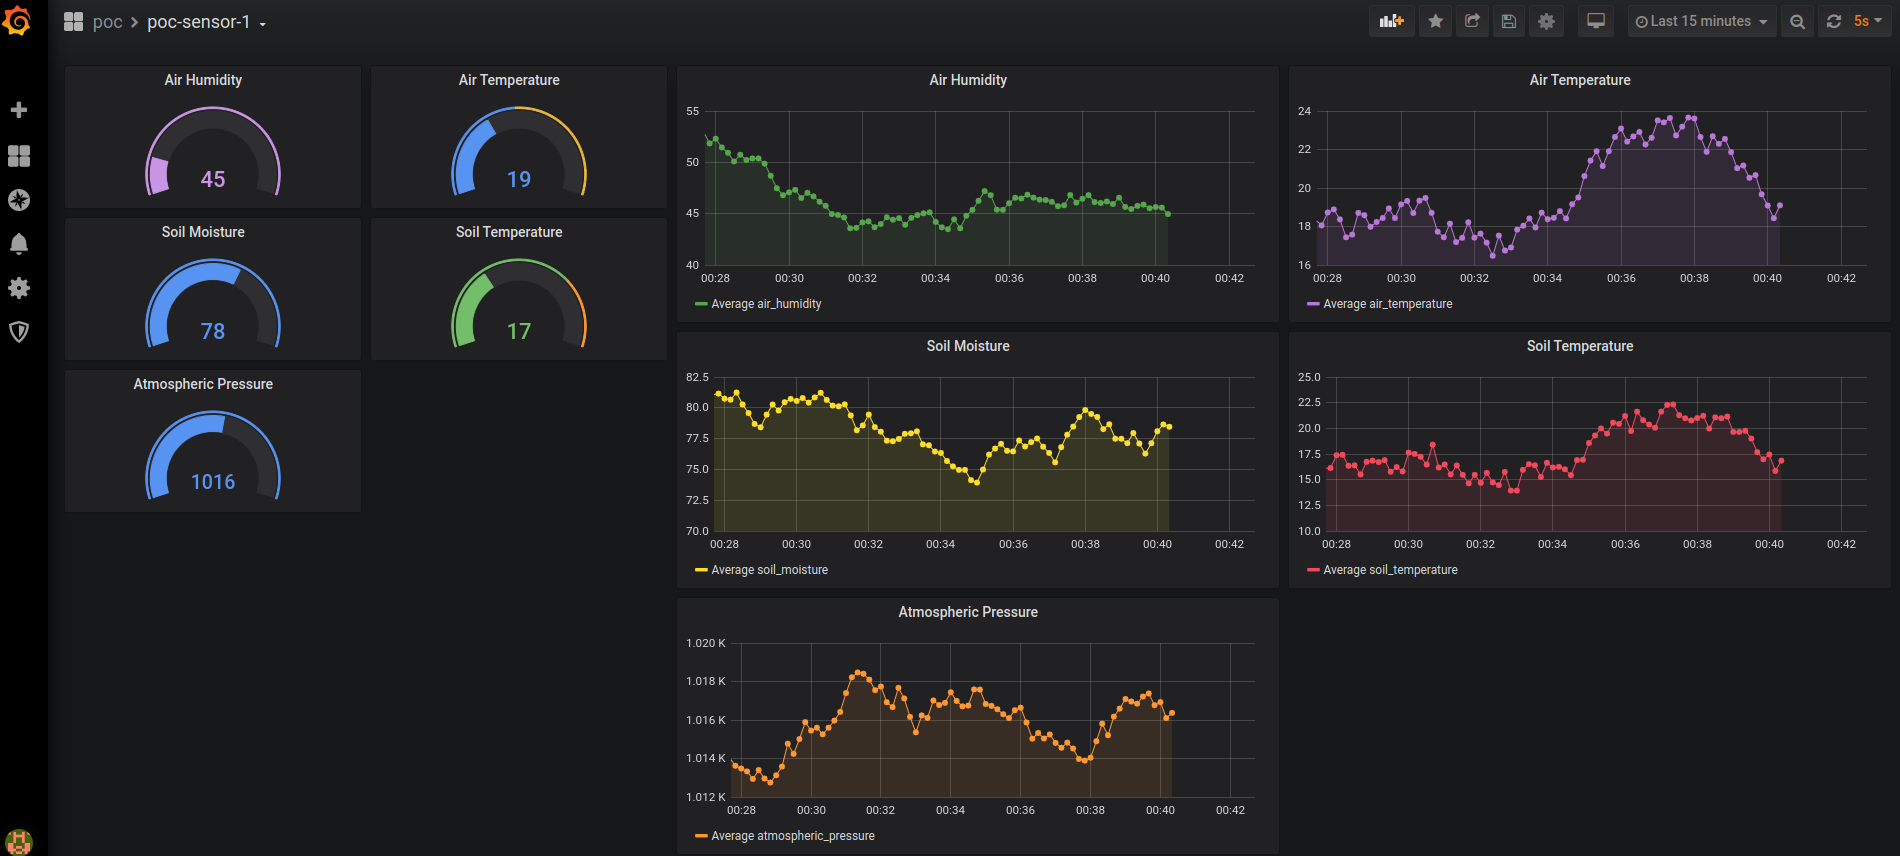
\includegraphics[width=0.9\columnwidth]{pruebaRepresentacion1.png}
    \caption{Interfaz de Grafana mostrando las métricas de uno de los sensores}
    \label{fig:pruebaRepresentacion1}
\end{figure}

\paragraph{}
La figura anterior no es más que un ejemplo de representación de las métricas de uno de los sensores IoT. Se ha configurado para mostrar los datos en tiempo real de las métricas uqe reportan los dispositivos hacia la nube. Se trata de un pequeño ejemplo de qué hacer con los datos una vez indexados en Elasticsearch.
\end{document}
